\chapter{Clustering}
In this chapter, we will explore a technique known as clustering. This represents our first foray into \textit{unsupervised} machine learning techniques. Unlike the previous four chapters, where we explored techniques that assumed a data set of inputs and targets, with the goal of eventually making predictions over unseen data, our data set will no longer contain explicit targets. Instead, these techniques are motivated by the goal of uncovering structure in our data. Identifying clusters of similar data points is a useful and ubiquitous unsupervised technique.

\section{Motivation}
The reasons for using an unsupervised technique like clustering are broad. We often don't have a specific task in mind; rather, we are trying to uncover more information about a potentially opaque data set. For clustering specifically, our unsupervised goal is to group data points that are similar.

There are many reasons why we might separate our data by similarity. For organizational purposes, it's convenient to have different classes of data. It can be easier for a human to sift through data if it's loosely categorized beforehand. It may be a preprocessing step for an inference method; for example, by creating additional features for a supervised technique. It can help identify which features make our data points most distinct from one another. It might even provide some idea of how many distinct data types we have in our set. 

This idea of data being `similar' means that we need some measure of \textit{distance} between our data points. While there are a variety of clustering algorithms available, the importance of this distance measurement is consistent between them.

Distance is meant to capture how `different' two data points are from each other. Then, we can use these distance measurements to determine which data points are similar, and thus should be clustered together. A common distance measurement for two data points $\textbf{x}$ and $\textbf{x}'$ is given by:
\begin{equation} \label{l2-distance}
	|| \textbf{x} - \textbf{x}' ||_{2} = \sqrt{\sum_{d=1}^{D} (\textbf{x}_{d} - \textbf{x}'_{d})^{2}}
\end{equation}
where $D$ is the dimensionality of our data. This is known as \textbf{L2} or \textbf{Euclidean distance}, and you can likely see the similarity to L2 regularization.

There are a variety of distance measurements available for data points living in a $D$-dimensional Euclidean space, but for other types of data (such as data with discrete features), we would need to select a different distance metric. Furthermore, the metrics we choose to use will have an impact on the final results of our clustering.

\begin{mlcube}{Clustering}
In unsupervised learning, the domain refers to the domain of the hidden variable z (which is analogous to y in supervised learning). In clustering, we have z's that represent the discrete clusters. Furthermore, the techniques that we explore in this chapter are fully unsupervised and non-probabilistic.
\begin{center}
    \begin{tabular}{c|c|c}
    \textit{\textbf{Domain}} & \textit{\textbf{Training}} & \textit{\textbf{Probabilistic}} \\
    \hline
    Discrete & Unsupervised & No \\
    \end{tabular}
\end{center}
\end{mlcube}

\subsection{Applications}
Here are a few specific examples of use cases for clustering:

\begin{enumerate}
    \item Determining the number of phenotypes in a population.
    \item Organizing images into folders according to scene similarity.
    \item Grouping financial data as a feature for anticipating extreme market events.
    \item Identifying similar individuals based on DNA sequences.
\end{enumerate}

As we mentioned above, there are different methods available for clustering. In this chapter, we will explore two of the most common techniques: K-Means Clustering and Hierarchical Agglomerative Clustering. We also touch on the flavors available within each of these larger techniques.

\section{K-Means Clustering}
The high level procedure behind K-Means Clustering (known informally as k-means) is as follows:

\begin{enumerate}
    \item Initialize cluster centers by randomly selecting points in our data set.
    \item Using a distance metric of your choosing, assign each data point to the closest cluster.
    \item Update the cluster centers based on your assignments and distance metric (for example, when using L2 distance, we update the cluster centers by averaging the data points assigned to each cluster).
    \item Repeat steps 2 and 3 until convergence.
\end{enumerate}

In the case where we are using the L2 distance metric, this is known as \textit{Lloyd's algorithm}, which we derive in the next section.

\subsection{Lloyd's Algorithm}
Lloyd's algorithm, named after Stuart P. Lloyd who first suggested the algorithm in 1957, optimizes our cluster assignments via a technique known as coordinate descent, which we will learn more about in later chapters.

\begin{derivation}{Lloyd's Algorithm Derivation}{lloyds-algorithm-derivation} \newline
	
	We begin by defining the objective used by Lloyd's algorithm. \newline \newline
	\underline{\textbf{Objective}} \newline
	The loss function for our current assignment of data points to clusters is given by:
	\begin{equation} \label{clustering-loss-fn}
		\mathcal{L}(\textbf{X}, \big\{\boldsymbol{\mu}\big\}_{k=1}^{K}, \big\{\textbf{r}\big\}_{n=1}^{N}) = \sum_{n=1}^{N} \sum_{k=1}^{K} r_{nk} ||\textbf{x}_{n} - \boldsymbol{\mu}_{k}||_2^{2}
	\end{equation}
	where $\textbf{X}$ is our $N \times D$ data set ($N$ is the number of data points and $D$ is the dimensionality of our data), $\big\{\boldsymbol{\mu}\big\}_{k=1}^{K}$ is the $K \times D$ matrix of cluster centers ($K$ is the number of clusters we chose), and $\big\{\textbf{r}\big\}_{n=1}^{N}$ is our $N \times K$ matrix of \textit{responsibility vectors}. These are one-hot encoded vectors (one per data point), where the 1 is in the position of the cluster to which we assigned the $n$th data point. \newline

	We now define the algorithmic portion of Lloyd's clustering procedure. \newline

	\underline{\textbf{Algorithm}} \newline
	We first adjust our responsibility vectors to minimize each data point's distance from its cluster center. Formally:
	\begin{equation} \label{responsibility-vector-update}
		r_{nk} = \begin{cases}
		 	= 1 & \text{if $k = \underset{k'}{\arg\min} ||\textbf{x}_{n} - \boldsymbol{\mu}_{k'}||$} \\
			= 0 & \text{otherwise} \\
		\end{cases}
	\end{equation}
	After updating our responsibility vectors, we now wish to minimize our loss by updating our cluster centers $\boldsymbol{\mu}_{k}$. The cluster centers which minimize our loss can be computed by taking the derivative of our loss with respect to $\boldsymbol{\mu}_{k}$, setting equal to 0, and solving for our new cluster centers $\boldsymbol{\mu}_{k}$:
	\begin{equation} \label{update-cluster-centers}
		\begin{aligned}
			\frac{\partial \mathcal{L}}{\partial \boldsymbol{\mu}_{k}} = -2 \sum_{n=1}^{N} r_{nk} (\textbf{x}_{n} - \boldsymbol{\mu}_{k}) \\
			\boldsymbol{\mu}_{k} = \frac{\sum_{n=1}^{N} r_{nk} \textbf{x}_{n}}{\sum_{n=1}^{N} r_{nk}}
		\end{aligned}
	\end{equation}
	Intuitively, this is the average of all the data points $\textbf{x}_{n}$ assigned to the cluster center $\boldsymbol{\mu}_{k}$. \newline

	We then update our responsibility vectors based on the new cluster centers, update the cluster centers again, and continue this cycle until we have converged on a stable set of cluster centers and responsibility vectors.
\end{derivation}

Note that while Lloyd's algorithm is guaranteed to converge, it is only guaranteed to converge to a locally optimal solution. Finding the globally optimal set of assignments and cluster centers is an NP-hard problem. As a result, a common strategy is to execute Lloyd's algorithm several times with different random initializations of cluster centers, selecting the assignment that minimizes loss across the different trials. Furthermore, to avoid nonsensical solutions due to scale mismatch between features (which would throw our Euclidean distance measurements off), it makes sense to standardize our data in a preprocessing step. This is as easy as subtracting the mean and dividing by the standard deviation across each feature.

\subsection{Example of Lloyd's}
For some more clarity on exactly how Lloyd's algorithm works, let's walk through an example.

\begin{example}{Lloyd's Algorithm Example}{lloyds-algorithm-example}
	We start with a data set of size $N=6$. Each data point is two-dimensional, with each feature taking on a value between -3 and 3. We also have a `Red' and `Green' cluster. Here is a table and graph of our data points, labelled A through F: \newline

	\begin{align*}
		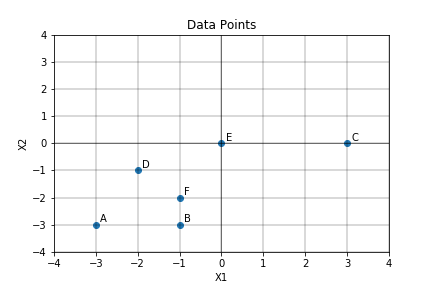
\includegraphics[width=0.5\paperwidth]{../Clustering/fig/start-points.png}
	\end{align*}

	\begin{align*}
	\begin{tabular}{lllll}
	\toprule
	{} & Coordinates & Dist. to Red & Dist. to Green & Cluster Assgn. \\
	\midrule
	A &    (-3, -3) &          n/a &            n/a &            n/a \\
	B &    (-1, -3) &          n/a &            n/a &            n/a \\
	C &      (3, 0) &          n/a &            n/a &            n/a \\
	D &    (-2, -1) &          n/a &            n/a &            n/a \\
	E &      (0, 0) &          n/a &            n/a &            n/a \\
	F &    (-1, -2) &          n/a &            n/a &            n/a \\
	\bottomrule
	\end{tabular}
	\end{align*} \newline

	Let's say we wish to have 2 cluster centers. We then randomly initialize those cluster centers by selecting two data points. Let's say we select B and F. We identify our cluster centers with a red and green `X' respectively:

	\begin{align*}
		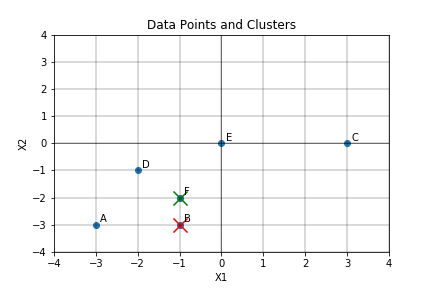
\includegraphics[width=0.5\paperwidth]{../Clustering/fig/start-clusters.png}
	\end{align*}

	We now begin Lloyd's algorithm by assigning each data point to its closest cluster center:

	\begin{align*}
		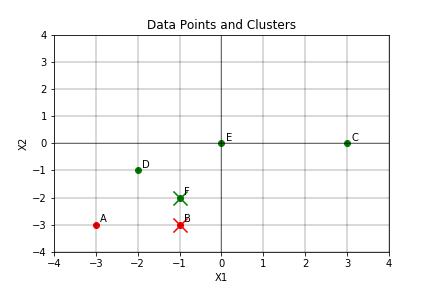
\includegraphics[width=0.5\paperwidth]{../Clustering/fig/assign-points.png}
	\end{align*}

	\begin{align*}
	\begin{tabular}{lllll}
	\toprule
	{} & Coordinates & Dist. to Red & Dist. to Green & Cluster Assgn. \\
	\midrule
	A &    (-3, -3) &         n/a &            n/a &              Red \\
	B &    (-1, -3) &         n/a &            n/a &              Red \\
	C &      (3, 0) &         n/a &            n/a &            Green \\
	D &    (-2, -1) &         n/a &            n/a &            Green \\
	E &      (0, 0) &         n/a &            n/a &            Green \\
	F &    (-1, -2) &         n/a &            n/a &            Green \\
	\bottomrule
	\end{tabular}
	\end{align*} \newline

	We then update our cluster centers by averaging the data points assigned to each:

	\begin{align*}
		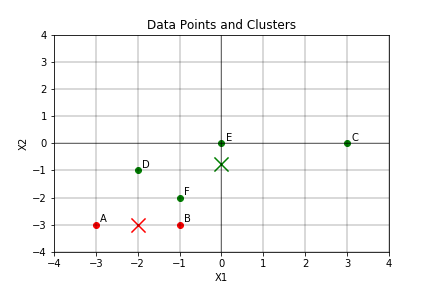
\includegraphics[width=0.5\paperwidth]{../Clustering/fig/update-clusters.png}
	\end{align*}

	\begin{align*}
	\begin{tabular}{lllll}
	\toprule
	{} & Coordinates & Dist. to Red & Dist. to Green & Cluster Assgn. \\
	\midrule
	A &    (-3, -3) &         2.00 &           2.24 &            Red \\
	B &    (-1, -3) &         0.00 &           1.00 &            Red \\
	C &      (3, 0) &         5.00 &           4.47 &          Green \\
	D &    (-2, -1) &         2.24 &           1.41 &          Green \\
	E &      (0, 0) &         3.16 &           2.24 &          Green \\
	F &    (-1, -2) &         1.00 &           0.00 &          Green \\
	\bottomrule
	\end{tabular}
	\end{align*}

	We proceed like this, updating our cluster centers and assignments, until convergence. At convergence, we've achieved these cluster centers and assignments:

	\begin{align*}
		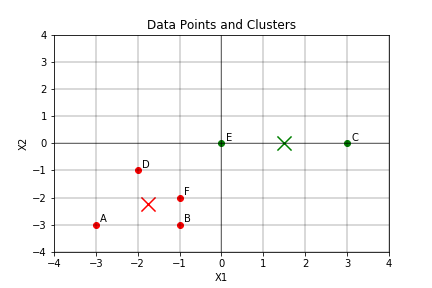
\includegraphics[width=0.5\paperwidth]{../Clustering/fig/final-points-and-clusters.png}
	\end{align*}

	\begin{align*}
	\begin{tabular}{lllll}
	\toprule
	{} & Coordinates & Dist. to Red & Dist. to Green & Cluster Assgn. \\
	\midrule
	A &    (-3, -3) &         1.46 &           5.41 &            Red \\
	B &    (-1, -3) &         1.06 &           3.91 &            Red \\
	C &      (3, 0) &         5.26 &           1.50 &          Green \\
	D &    (-2, -1) &         1.27 &           3.64 &            Red \\
	E &      (0, 0) &         2.85 &           1.50 &          Green \\
	F &    (-1, -2) &         0.79 &           3.20 &            Red \\
	\bottomrule
	\end{tabular}
	\end{align*}

	Where our red cluster is at (-1.75, -2.25) and our green cluster is at (1.5 ,  0). Note that for this random initialization of cluster centers, we deterministically identified the locally optimal set of assignments and cluster centers. For a specific initialization, running Lloyd's algorithm will always identify the same set of assignments and cluster centers. However, different initializations will produce different results. For example, consider when we initialize our cluster centers at E and C. 
\end{example}

\subsection{Number of Clusters}
You may have wondered about a crucial, omitted detail: how do we choose the proper number of clusters for our data set? There doesn't actually exist a `correct' number of clusters. The fewer clusters we have, the larger our loss will be, and as we add more clusters, our loss will get strictly smaller. That being said, there is certainly a tradeoff to be made here.

Having a single cluster is obviously useless - we will group our entire data set into the same cluster. Having $N$ clusters is equally useless - each data point gets its own cluster.

One popular approach to identifying a good number of clusters is to perform K-Means with a varying number of clusters, and then to plot the number of clusters against the loss. Typically, that graph will look like Figure \ref{fig:knee}.

\begin{figure}
    \centering
    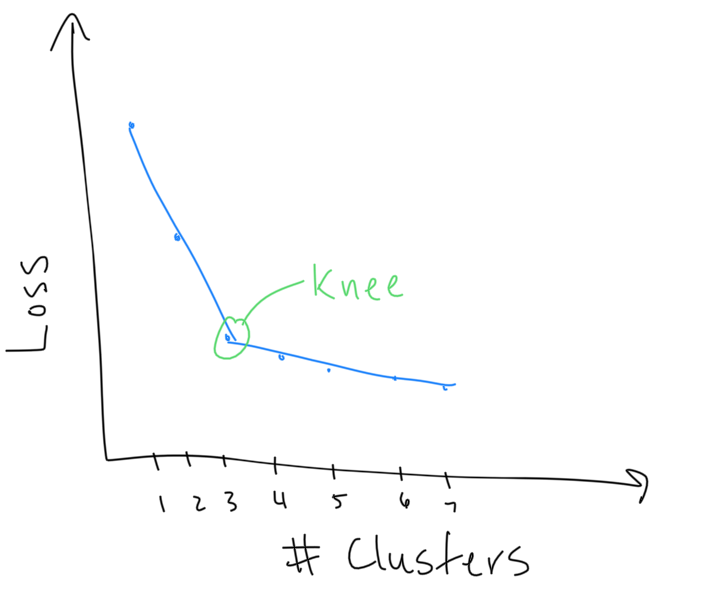
\includegraphics[width=0.5\paperwidth]{../Clustering/fig/knee.png}
    \caption{Finding the Knee.}
    \label{fig:knee}
\end{figure}

Notice that at $x=3$ clusters, there appears to be a slight bend in the decrease of our loss. This is often called the \textbf{knee} (or elbow), and it is common to choose the number of clusters to be where the knee occurs.

Intuitively, the idea here is that up to a certain point, adding another cluster significantly decreases the loss by more properly grouping our data points. However, eventually the benefit of adding another cluster stops being quite so significant. At this point, we have identified a natural number of groups for our data set.

\subsection{Initialization and K-Means++}
Up until now, we have assumed that we should randomly initialize our cluster centers and execute Lloyd's algorithm until convergence. We also suggested that since Lloyd's algorithm only produces a local minimum, it makes sense to perform several random initializations before settling on the most optimal assignment we've identified.

While this is a viable way to perform K-Means, there are other ways of initializing our original cluster centers that can help us find more optimal results without needing so many random initializations. One of those techniques is known as \textbf{K-Means++}.

The idea behind K-Means++ is that our cluster centers will typically be spread out when we've reached convergence. As a result, it might not make sense to initialize those cluster centers in an entirely random manner. For example, Figure \ref{fig:bad-init} would be a poor initialization.

\begin{figure}
    \centering
    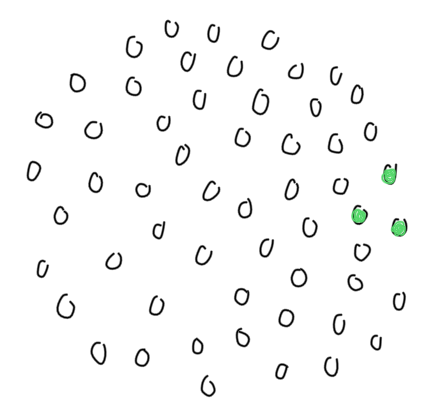
\includegraphics[width=0.5\paperwidth]{../Clustering/fig/bad-initialization.png}
    \caption{Bad Cluster Initialization.}
    \label{fig:bad-init}
\end{figure}

We would much rather start with a random initialization that looks like Figure \ref{fig:good-init}.

\begin{figure}
    \centering
    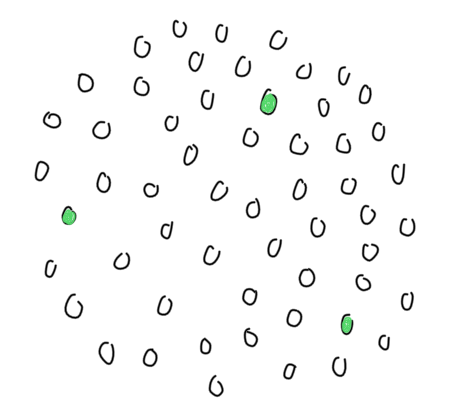
\includegraphics[width=0.5\paperwidth]{../Clustering/fig/good-initialization.png}
    \caption{Good Cluster Initialization.}
    \label{fig:good-init}
\end{figure}

We can use the hint that we want our cluster centers somewhat spread out to find a better random initialization. This is where the initialization algorithm presented by K-Means++ comes in.

For K-Means++, we choose the first cluster center by randomly selecting a point in our data set, same as before. However, for all subsequent cluster center initializations, we select points in our data set with probability proportional to the squared distance from their nearest cluster center. The effect of this is that we end up with a set of initializations that are relatively far from one another, as in Figure \ref{fig:good-init}.

\subsection{K-Medoids Alternative}
Recall that in the cluster center update step (Equation \ref{update-cluster-centers}) presented in the derivation of Lloyd's algorithm, we average the data points assigned to each cluster to compute the new cluster centers. Note that in some cases, this averaging step doesn't actually make sense (for example, if we have categorical variables as part of our feature set). In these cases, we can use an alternative algorithm known as \textbf{K-Medoids}. The idea behind K-Medoids is simple: instead of averaging the data points assigned to that cluster, update the new cluster center to be the data point assigned to that cluster which is most like the others.

\section{Hierarchical Agglomerative Clustering}
The motivating idea behind K-Means was that we could use a distance measurement to assign data points to a fixed number of clusters, iteratively improving our assignments and cluster locations until convergence.

Moving on to Hierarchical Agglomerative Clustering (also known as \textbf{HAC} - pronounced `hack'), the motivating idea is instead to group data from the bottom up. This means every data point starts as its own cluster, and then we merge clusters together based on a distance metric that we define. This iterative merging allows us to construct a tree over our data set that describes relationships between our data. These trees are known as \textit{dendrograms}, with an example found in Figure \ref{fig:dendrogram-example}. Notice that the individual data points are the leaves of our tree, and the trunk is the cluster that contains the entirety of our data set. The y-axis of the dendrogram represents the distance between clusters.

\begin{figure}
    \centering
    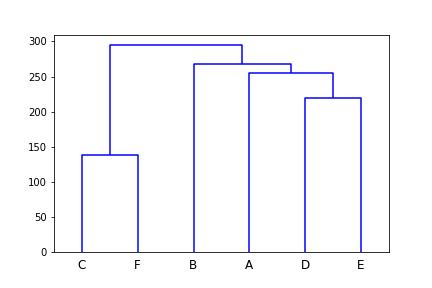
\includegraphics[width=0.5\paperwidth]{../Clustering/fig/dendrogram-example.png}
    \caption{Dendrogram Example.}
    \label{fig:dendrogram-example}
\end{figure}

We now formally define the HAC algorithm, and in the process, explain how we construct such a tree.

\subsection{HAC Algorithm}
\begin{enumerate}
    \item Start with $N$ clusters, one for each data point.
    \item Measure the distance between clusters. This will require an inter-cluster distance measurement that we will define shortly.
    \item Merge the two `closest' clusters together, reducing the number of clusters by 1. Record the distance between these two merged clusters.
    \item Repeat step 2 until we're left with only a single cluster.
\end{enumerate}

In the remainder of the chapter, we'll describe this procedure in greater detail (including how to measure the distance between clusters), explain the clustering information produced by the tree, and discuss how HAC differs from K-Means. But first, to make this algorithm a little more clear, let's perform HAC one step at a time on a toy data set, constructing the dendrogram as we go.

\begin{example}{HAC Algorithm Example}{hac-algo-example}
Let's say we have a data set of five points A, B, C, D, E that we wish to perform HAC on. These points will simply be scalar data that we can represent on a number line. We start with 5 clusters and no connections at all:

\begin{align*}
	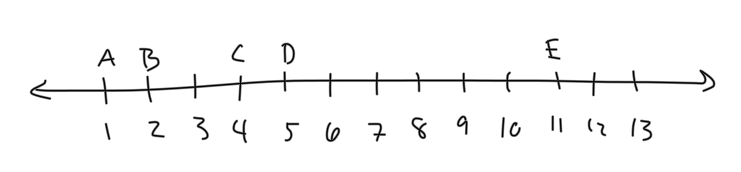
\includegraphics[width=0.5\paperwidth]{../Clustering/fig/number-line.png}
\end{align*}

We find the closest two clusters to merge first. A and B are nearest (it's actually tied with C and D, but we can arbitrarily break these ties), so we start by merging them. Notice that we also annotate the distance between them in the tree, which in this case is 1:

\begin{align*}
	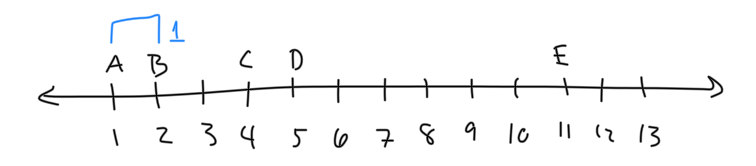
\includegraphics[width=0.5\paperwidth]{../Clustering/fig/a-b-merged.png}
\end{align*}

We now have four clusters: (A, B), C, D, and E. We again find the closest two clusters, which in this case is C and D:

\begin{align*}
	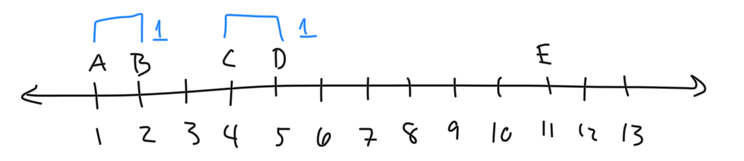
\includegraphics[width=0.5\paperwidth]{../Clustering/fig/c-d-merged.png}
\end{align*}

We now have three remaining clusters: (A, B), (C, D), and E. We proceed as before, identifying the two closest clusters to be (A, B) and (C, D). Merging them:

\begin{align*}
	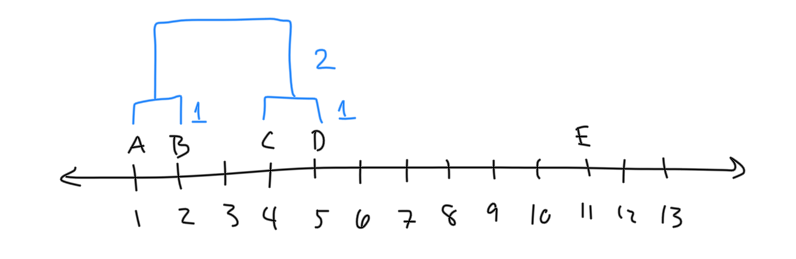
\includegraphics[width=0.5\paperwidth]{../Clustering/fig/a-b-c-d-merged.png}
\end{align*}

Finally we are left with two clusters: (A, B, C, D) and E. The remaining two clusters are obviously the closest together, so we merge them:

\begin{align*}
	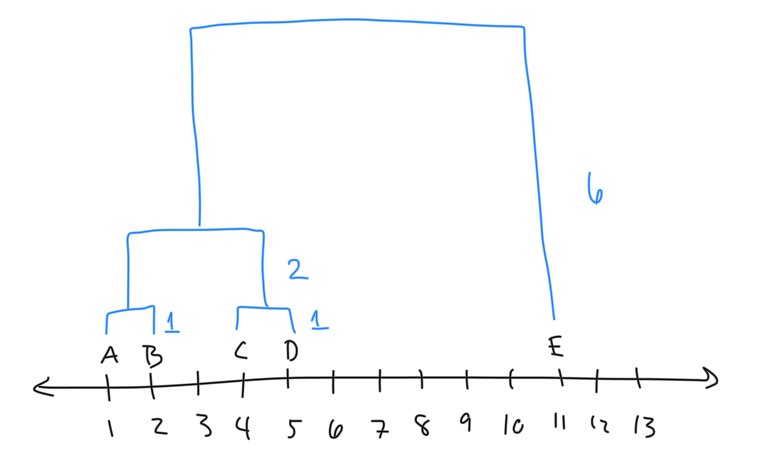
\includegraphics[width=0.5\paperwidth]{../Clustering/fig/a-b-c-d-e-merged.png}
\end{align*}

At this point there is only a single cluster. We have constructed our tree and are finished with HAC.
\end{example}

Notice how the distance between two merged clusters manifests itself through the height of the dendrogram where they merge (which is why we tracked those distances as we constructed the tree). Notice also that we now have many layers of clustering: if we're only only interested in clusters whose elements are at least $k$ units away from each other, we can `cut' the dendrogram at that height and examine all the clusters that exist below that cut point.

Finally, we need to handle the important detail of how to compute the distance between clusters. In the preceding example, we designated the distance between two clusters to be the minimum distance between any two data points in the clusters. This is what is known as the \textbf{Min-Linkage Criterion}. However, there are certainly other ways we could have computed the distance between clusters, and using a different distance measurement can produce different clustering results. We now turn to these different methods and the properties of clusters they produce.

\subsection{Linkage Criterion}
Here are a few of the most common linkage criteria.

\subsubsection{Min-Linkage Criteria}
We've already seen the Min-Linkage Criterion in action from the previous example. Formally, the criterion says that the distance $d_{C, C'}$ between each cluster pair $C$ and $C'$ is given by
\begin{equation} \label{min-linkage-crit}
	d_{C, C'} = \underset{k, k'}{\min} || \textbf{x}_{k} - \textbf{x}_{k'} ||
\end{equation}
where $\textbf{x}_{k}$ are data points in cluster $C$ and $\textbf{x}_{k'}$ are data points in cluster $C'$. After computing these pairwise distances, we choose to merge the two clusters that are closest together.

\subsubsection{Max-Linkage Criterion}
We could also imagine defining the distance $d_{C, C'}$ between two clusters as being the distance between the two points that are farthest apart in each cluster. This is known as the Max-Linkage Criterion. The distance between two clusters is then given by:
\begin{equation} \label{max-linkage-crit}
	d_{C, C'} = \underset{k, k'}{\max} || \textbf{x}_{k} - \textbf{x}_{k'} ||
\end{equation}
As with the Min-Linkage Criterion, after computing these pairwise distances, we choose to merge the two clusters that are closest together.

\readernote{Be careful not to confuse the linkage criterion with which clusters we choose to merge. We \textbf{always} merge the clusters that have the smallest distance between them. How we compute that distance is given by the linkage criterion.}

\subsubsection{Average-Linkage Criterion}
The Average-Linkage Criterion averages the pairwise distance between each point in each cluster. Formally, this is given by:
\begin{equation} \label{avg-linkage-crit}
	d_{C, C'} = \frac{1}{K K'} \sum_{k=1}^{K} \sum_{k'=1}^{K'} || \textbf{x}_{k} - \textbf{x}_{k'} ||
\end{equation}

\subsubsection{Centroid-Linkage Criterion}
The Centroid-Linkage Criterion uses the distance between the centroid of each cluster (which is the average of the data points in a cluster). Formally, this is given by:
\begin{equation} \label{cent-linkage-crit}
	d_{C, C'} = || \frac{1}{K} \sum_{k=1}^{K} \textbf{x}_{k} - \frac{1}{K'} \sum_{k'=1}^{K'} \textbf{x}_{k'} ||
\end{equation}

\subsubsection{Different Linkage Criteria Produce Different Clusterings}
It's important to note that the linkage criterion you choose to use will influence your final clustering results. For example, the min-linkage criterion tends to produce `stringy' clusters, while the max-linkage criterion tends to produce more compact clusters. You can see the difference between the results of these two linkage criteria in Figure \ref{fig:diff-linkage-criteria}.

\begin{figure}
    \centering
    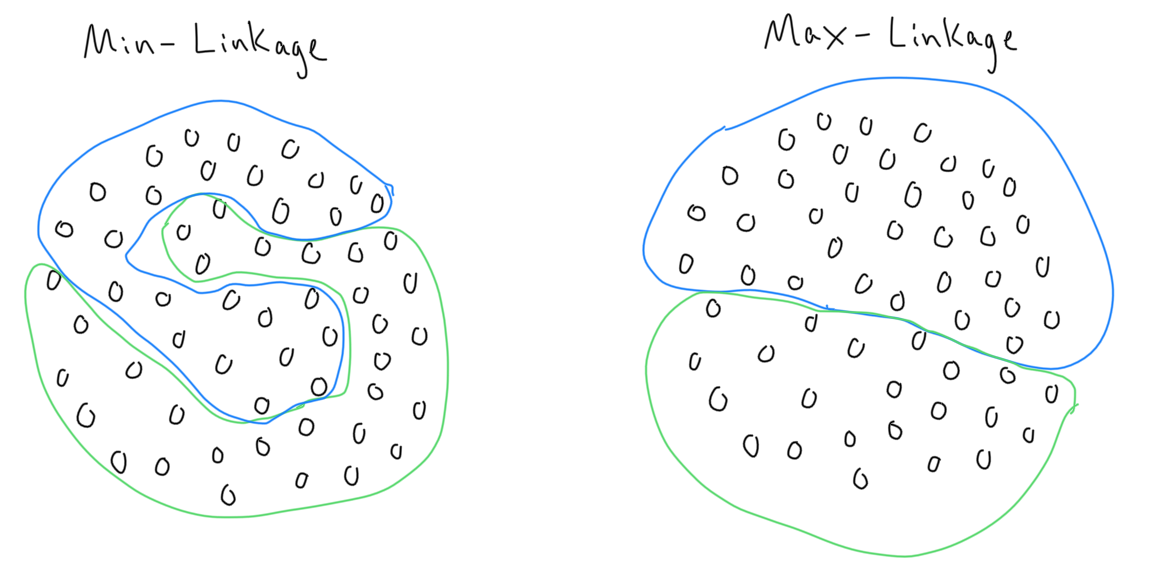
\includegraphics[width=0.5\paperwidth]{../Clustering/fig/diff-linkage-criteria.png}
    \caption{Different Linkage Criteria.}
    \label{fig:diff-linkage-criteria}
\end{figure}

\readernote{You should convince yourself of the different flavors of linkage criteria. For example, when using the min-linkage criterion, we get these `stringy' results because we're most inclined to extend existing clusters by grabbing whichever data points are closest.}

\subsection{How HAC Differs from K-Means}
Now that we're aware of two distinct clustering techniques and their variants, we consider the differences between the two methods.

First of all, there is a fundamental difference in determinism between HAC and K-Means. In general, K-Means incurs a certain amount of randomness and needs to be run multiple times to ensure a good result. On the other hand, once you've selected a linkage criterion for HAC, the clusters you calculate are deterministic. You only need to run HAC a single time.

Another difference between HAC and K-Means comes from the assumptions we make. For K-Means, we need to specify the number of clusters up front before running our algorithm, potentially using something like the knee-method to decide on the number of clusters. On the other hand, you don't need to assume anything to run HAC, which simplifies its usage. However, the downside for HAC is that when you wish to present your final clustering results, you need to decide on the max distance between elements in each cluster (so that you can cut the dendrogram).

The fact that you need to make a decision about where to cut the dendrogram means that running HAC once gives you several different clustering options. Furthermore, the dendrogram in and of itself can be a useful tool for visualizing data. We don't get the same interactivity from K-Means clustering.

\readernote{We often use dendrograms to visualize evolutionary lineage.}